%-----------------------------------------------------------------------------%
\chapter{\babDua}
\label{bab:2}
%-----------------------------------------------------------------------------%

%-----------------------------------------------------------------------------%
\section{Knowledge Graph}
\label{sec:knowledgeGraph}
%-----------------------------------------------------------------------------%

%-----------------------------------------------------------------------------%
\subsection{Triple}
\label{sec:triple}
%-----------------------------------------------------------------------------%
\textit{Triple} merupakan tuple dengan yang terdiri dari tiga elemen yaitu subject, object, dan predikat. 
Terdapat dua representasi elemen dari \textit{triple}, yaitu URI dan literal. 
Resource merupakan URI yang dapat digunakan sebagai subject dan object. Property merupakan URI yang dapat digunakan sebagai predikat. 
Dan literal hanya dapat digunakan sebagai object. 
\textit{Knowledge graph} dibangun dari himpunan \textit{triple}.
Selanjutnya \textit{resource} akan dinotasikan dalam \resource{teks monospace berwarna biru} dan \textit{predicate} akan dinotasikan dalam \predicate{teks monospace berwarna merah}.

\begin{figure}
\centering
    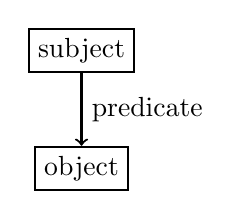
\begin{tikzpicture}[node distance={15mm}, thick, main/.style = {draw, rectangle}] 
        \node[main] (subject) {\resource{subject}};
        \node[main] (object) [below of=subject] {\resource{object}};
        \draw[->] (subject) -- node[midway, right] {\predicate{predicate}} (object);
    \end{tikzpicture} 
\caption{Ilustrasi \textit{triple}}
\end{figure} 


%-----------------------------------------------------------------------------%
\section{Jenis Peraturan Perundang-undangan}
\label{sec:jenisPeraturanPerundangUndangan}
%-----------------------------------------------------------------------------%
Terdapat beberapa jenis peraturan perundang-undangan.
Setiap dokumen peraturan perundang-undangan adalah resource, dan memiliki susunan URI yang berbeda.
Berikut adalah jenis peraturan perundang-undangan:
\begin{itemize}
    \item Undang-Undang
    \item Peraturan Pemerintah Pengganti Undang-Undang
    \item Peraturan Pemerintah
    \item Peraturan Presiden
    \item Peraturan Menteri
    \item Peraturan Lembaga
    \item Peraturan Daerah
\end{itemize}

%-----------------------------------------------------------------------------%
\subsection{Undang-Undang}
\label{sec:undangUndang}
%-----------------------------------------------------------------------------%
\begin{figure}
\[
    \defbox{ex.org/dokumen/uu/}{prefix}{gray}
    \defbox{2003/}{tahun}{blue}
    \defbox{13/}{nomor}{red}
\]
\caption{Contoh URI untuk undang-undang nomor 13 tahun 2003}
\end{figure}

%-----------------------------------------------------------------------------%
\subsection{Peraturan Daerah}
\label{sec:peraturanDaerah}
%-----------------------------------------------------------------------------%
\begin{figure}
\[
    \defbox{ex.org/dokumen/perda/}{prefix}{gray}
    \defbox{provinsi\_dki\_jakarta/}{kode daerah}{brown}
    \defbox{2020/}{tahun}{blue}
    \defbox{33/}{nomor}{red}
\]
\caption{Contoh URI untuk peraturan gubernur DKI Jakarta nomor 33 tahun 2020}
\end{figure}

%-----------------------------------------------------------------------------%
\section{Komponen Dokumen Peraturan Perundang-undangan}
\label{sec:komponenDokumenPeraturanPerundangUndangan}
%-----------------------------------------------------------------------------%
Dokumen terdiri dari komponen dokumen. Komponen dokumen diantaranya adalah \resource{bab}, \resource{bagian}, \resource{paragraf}, \resource{pasal}, \resource{ayat}, dan \resource{point}. Setiap komponen dokumen merupakan resource, dan memiliki URI. URI sebuah komponen didahului oleh URI dokumennya. Berikut adalah relasi antara komponen dokumen yang disediakan.

\begin{figure}
\centering
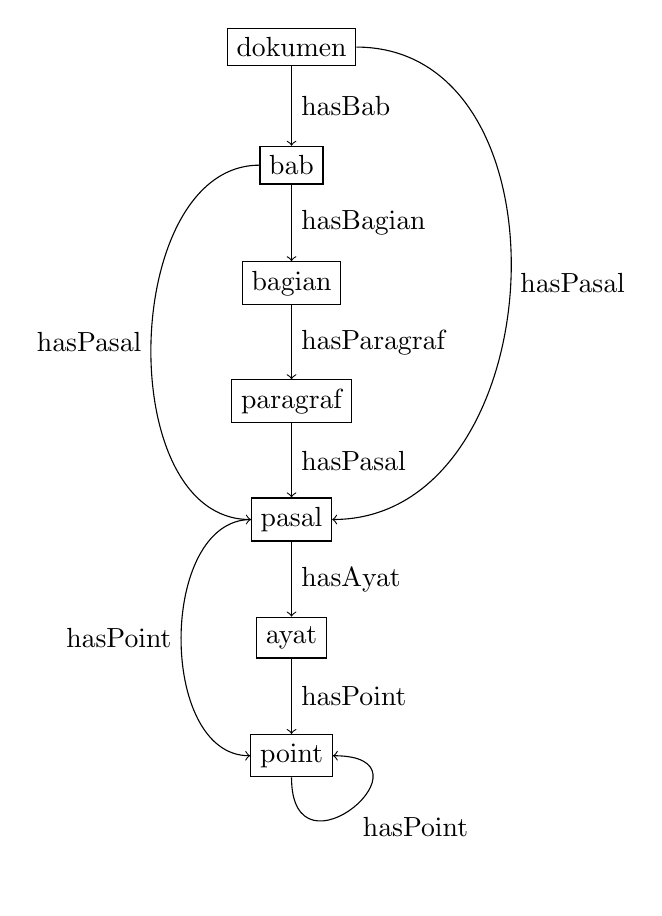
\begin{tikzpicture}[node distance={15mm}, main/.style = {draw, rectangle}] 
    \node[main] (doc) {\resource{dokumen}}; 
    \node[main] (bab) [below of=doc] {\resource{bab}};
    \node[main] (bagian) [below of=bab] {\resource{bagian}};
    \node[main] (paragraf) [below of=bagian] {\resource{paragraf}};
    \node[main] (pasal) [below of=paragraf] {\resource{pasal}};
    \node[main] (ayat) [below of=pasal] {\resource{ayat}};
    \node[main] (point) [below of=ayat] {\resource{point}};
    \draw[->] (doc) -- node[midway, right] {\predicate{hasBab}} (bab);
    \draw[->] (bab) -- node[midway, right] {\predicate{hasBagian}} (bagian);
    \draw[->] (bagian) -- node[midway, right] {\predicate{hasParagraf}} (paragraf);
    \draw[->] (paragraf) -- node[midway, right] {\predicate{hasPasal}} (pasal);
    \draw[->] (doc) to [in=0, out=0, looseness=1.2] node[midway, right] {\predicate{hasPasal}} (pasal);
    \draw[->] (bab) to [in=180, out=180] node[midway, left] {\predicate{hasPasal}} (pasal);
    \draw[->] (pasal) -- node[midway, right] {\predicate{hasAyat}} (ayat);
    \draw[->] (pasal) to [in=180, out=180] node[midway, left] {\predicate{hasPoint} } (point);
    \draw[->] (ayat) -- node[midway, right] {\predicate{hasPoint}} (point);
    \draw[->] (point) to [in=0, out=270, looseness=6] node[midway, below right]  {\predicate{hasPoint}} (point);
\end{tikzpicture} 
\caption{\textit{Resource} komponen dokumen dan \textit{property} antar komponen}
\end{figure} 

%-----------------------------------------------------------------------------%
\subsection{Bab}
\label{sec:bab}
%-----------------------------------------------------------------------------%
\begin{figure}
\centering
\[
    \defbox{ex.org/dokumen/uu/2003/13/}{URI dokumen}{gray}
    bab/
    \defbox{2/}{no. bab}{blue}
\]
\caption{Contoh URI untuk bab 2}
\end{figure}

%-----------------------------------------------------------------------------%
\subsection{Bagian}
\label{sec:bagian}
%-----------------------------------------------------------------------------%
\begin{figure}
\[
    \defbox{ex.org/dokumen/uu/2003/13/}{URI dokumen}{gray}
    bab/
    \defbox{10/}{no. bab}{blue}
    bagian/
    \defbox{3/}{no. bagian}{brown}
\]
\caption{Contoh URI untuk bab 10 bagian 3}
\end{figure}

%-----------------------------------------------------------------------------%
\subsection{Paragraf}
\label{sec:paragraf}
%-----------------------------------------------------------------------------%
\begin{figure}
\[
    \defbox{ex.org/dokumen/uu/2003/13/}{URI dokumen}{gray}
    bab/
    \defbox{7/}{no. bab}{blue}
    bagian/
    \defbox{4/}{no. bagian}{brown}
    paragraf/
    \defbox{5/}{no. pasal}{red}
\]
\caption{Contoh URI untuk bab 10 bagian 4 paragraf 5}
\end{figure}

%-----------------------------------------------------------------------------%
\subsection{Pasal}
\label{sec:pasal}
%-----------------------------------------------------------------------------%
\begin{figure}
\[
    \defbox{ex.org/dokumen/uu/2003/13/}{URI dokumen}{gray}
    pasal/
    \defbox{1/}{no. pasal}{purple}
\]
\caption{Contoh URI untuk pasal 1}
\end{figure}

%-----------------------------------------------------------------------------%
\subsection{Ayat}
\label{sec:ayat}
%-----------------------------------------------------------------------------%
\begin{figure}
\[
    \defbox{ex.org/dokumen/uu/2003/13/}{URI dokumen}{gray}
    pasal/
    \defbox{1/}{no. pasal}{purple}
    ayat/
    \defbox{8/}{no. ayat}{blue}
\]
\caption{Contoh URI untuk pasal 1 ayat 8}
\end{figure}

%-----------------------------------------------------------------------------%
\subsection{Huruf}
\label{sec:huruf}
%-----------------------------------------------------------------------------%
\begin{figure}
\[
    \defbox{ex.org/dokumen/uu/2003/13/}{URI dokumen}{gray}
    pasal/
    \defbox{1/}{no. pasal}{purple}
    ayat/
    \defbox{8/}{no. ayat}{blue}
    point/
    \defbox{g/}{huruf}{brown}
\]
\caption{Contoh URI untuk pasal 1 ayat 8 huruf g}
\end{figure}

\begin{figure}
\[
    \defbox{ex.org/dokumen/uu/2003/13/}{URI dokumen}{gray}
    pasal/
    \defbox{1/}{no. pasal}{purple}
    ayat/
    \defbox{8/}{no. ayat}{blue}
    point/
    \defbox{g/}{huruf 1}{brown}
    point/
    \defbox{3/}{huruf 2}{brown}
\]
\caption{Contoh URI untuk pasal 1 ayat 8 huruf g-3}
\end{figure}


%-----------------------------------------------------------------------------%
\section{Pekerjaan Terkait}
\label{sec:pekerjaanTerkait}
%-----------------------------------------------------------------------------%


%-----------------------------------------------------------------------------%
\subsection{European Legislation Identifier (ELI)}
\label{sec:eli}
%-----------------------------------------------------------------------------%
ELI merupakan sistem untuk membuat peraturan perundang-undangan tersedia secara daring dalam format terstandardisasi, sehingga dapat diakses dan digunakan oleh berbagai instansi. ELI dibangun berdasarkan persetujuan antara negara-negara EU. ELI memberikan spesifikasi untuk hal-hal berikut:
\begin{itemize}
    \item URI untuk informasi peraturan perundang-undangan.
    \item Metadata yang mendeskripsikan informasi peraturan perundang-undangan.
\end{itemize}
